\documentclass[tikz,dvisvgm]{standalone}
\usetikzlibrary{arrows.meta, calc, decorations.pathreplacing,
                ext.paths.ortho, positioning, quotes}
\makeatletter
\tikzset{phantom node/.code=\tikz@addoption{\expandafter\let\csname pgf@sh@boxes@\tikz@shape\endcsname\pgfutil@empty}}
\makeatother
\tikzset{
  shadowed node xshift/.initial=1.5ex, shadowed node yshift/.initial=1ex, shadowed node list/.initial={2, 1},
  pics/shadowed node/.default=\pgfkeysvalueof{/tikz/shadowed node list},
  shadowed node/.pic={
    \foreach[expand list] \elem in {#1}
      \scoped[transparency group, shadowed node calculation={\elem}]
        \node[style/.expand once=\tikzpictextoptions, phantom node,
              xshift={\elem*\pgfkeysvalueof{/tikz/shadowed node xshift}},
              yshift={\elem*\pgfkeysvalueof{/tikz/shadowed node yshift}}] (-\elem) {\tikzpictext};
    \node[alias=-0, style/.expand once=\tikzpictextoptions] () {\tikzpictext};},
  set shadowed node calculation parameter/.style={shadowed node calculation/.style={opacity={(#1-##1+1)/(#1+1)}}},
  set shadowed node calculation parameter=2,
  overshoot line to/.style={to path={($(\tikztostart)!-(#1)!(\tikztotarget)$)--($(\tikztotarget)!-(#1)!(\tikztostart)$)\tikztonodes}},
  edges have transparency group/.style={execute at begin to={\scope[transparency group,#1]}, execute at end to=\endscope}}
\begin{document}
\sffamily
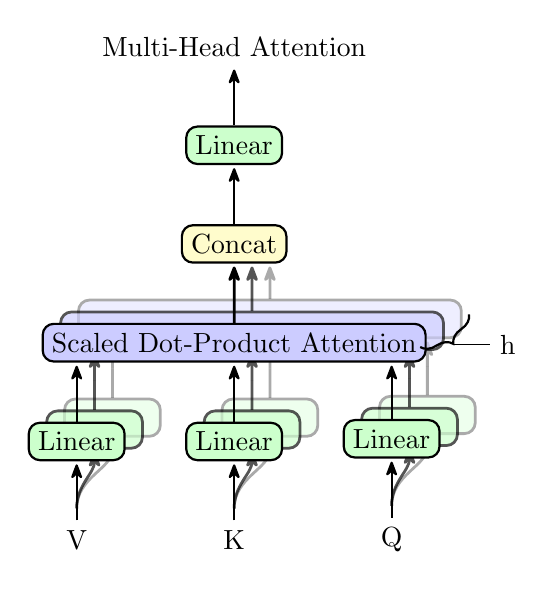
\begin{tikzpicture}[
  thick, x=2cm, node distance=7.5mm,
  n/.style={rounded corners, draw, fill={#1!20}},
  > = {Stealth[round, sep]}]
  % By default, all nodes/pics/edges are placed "in front of path"
  % here, the actual path is empty (edges create their own path)
  \node foreach[count=\i] \t in {V, K, Q} (VKQ-\i) at (\i, 0) {\t}
  pic foreach \i in {1, 2, 3}
    ["Linear" n=green, above=of VKQ-\i] (Linear-\i) {shadowed node}
  pic["Scaled Dot-Product Attention" n=blue, above = of Linear-2]
  (Attention) {shadowed node}
  node[above = of Attention, n = yellow] (Concat) {Concat}
  node[above = of Concat,    n = green]  (Linear) {Linear}
  node[above = of Linear]                (MHAtt)  {Multi-Head Attention}
    %
    [->, ortho/install shortcuts]
  foreach \i in {1, 2, 3}{
      (VKQ-\i) edge coordinate [pos=.2] (@) (Linear-\i)
      (Linear-\i) edge[|*] (Attention)
      foreach \j in {2, 1}{
          [
              edges have transparency group={shadowed node calculation=\j},
              behind path % this edges should be behind the other nodes/pics
            ]
          (@) edge[out=90, in=-90] (Linear-\i-\j)
          [in front of path] % split the following path midway (→ @@)
          (Linear-\i-\j) edge[path only, |*] coordinate (@@) (Attention-\j)
          edge[-] (@@)                % draw the first half on top
          [behind path] (@@) edge[|*] (Attention-\j) % and the second behind
        }
    }
  foreach \i in {0, 1, 2}{
      [edges have transparency group={shadowed node calculation=\i}]
      (Attention-\i) edge[|*] (Concat)
    }
  (Concat) edge (Linear)
  (Linear) edge (MHAtt);
  \draw[decorate, decoration = {name = brace, amplitude = 2mm}]
  (Attention-2.east) to[overshoot line to=1mm] (Attention.east);
  \path[every pin edge/.style={black, thin}] coordinate [pin=right:h] ()
  at ($(Attention-2.east)!.5!(Attention.east)!2mm+.5\pgflinewidth!90:(Attention.east)$);
  % \draw[
  % arrows={[arc=135]}, arrows={Hooks[left]-Hooks[right]},
  % s/.style={shift={(.75mm,-1mm)}}]
  % ([s]Attention-2.east) to[overshoot line to=2mm] coordinate(@) ([s]Attention.east);
  % \path[every pin edge/.style={black, thin}] node also[pin=right:h](@);
\end{tikzpicture}
\end{document}
